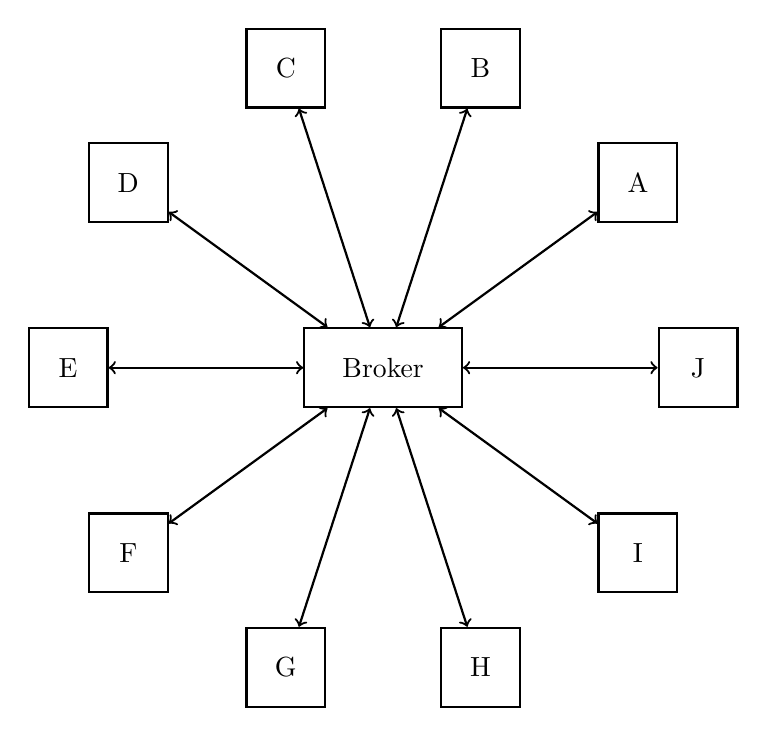
\begin{tikzpicture}[thick]

  % Draw nodes
  \foreach \t [count=\a] in {A,B,C,D,E,F,G,H,I,J}{
    \draw (\a*360/10: 4cm) node(\t)[draw,rectangle,minimum width=1cm,minimum height=1cm]{\t};
    }

  \begin{scope}
    \node(Broker) [draw,rectangle,minimum width=2cm,minimum height=1cm]{Broker};
  \end{scope}

  % Draw connections
  \foreach \t [count=\a] in {A,B,C,D,E,F,G,H,I,J}{
    \draw[<->] (\t) edge (Broker);
    }

\end{tikzpicture}
